
% Default to the notebook output style

    


% Inherit from the specified cell style.




    
\documentclass{article}

    
    
    \usepackage{graphicx} % Used to insert images
    \usepackage{adjustbox} % Used to constrain images to a maximum size 
    \usepackage{color} % Allow colors to be defined
    \usepackage{enumerate} % Needed for markdown enumerations to work
    \usepackage{geometry} % Used to adjust the document margins
    \usepackage{amsmath} % Equations
    \usepackage{amssymb} % Equations
    \usepackage[mathletters]{ucs} % Extended unicode (utf-8) support
\usepackage[spanish]{babel}
\usepackage[utf8]{inputenc}
    \usepackage{fancyvrb} % verbatim replacement that allows latex
    \usepackage{grffile} % extends the file name processing of package graphics 
                         % to support a larger range 
    % The hyperref package gives us a pdf with properly built
    % internal navigation ('pdf bookmarks' for the table of contents,
    % internal cross-reference links, web links for URLs, etc.)
    \usepackage{hyperref}
    \usepackage{longtable} % longtable support required by pandoc >1.10
    \usepackage{booktabs}  % table support for pandoc > 1.12.2
    

    
    
    \definecolor{orange}{cmyk}{0,0.4,0.8,0.2}
    \definecolor{darkorange}{rgb}{.71,0.21,0.01}
    \definecolor{darkgreen}{rgb}{.12,.54,.11}
    \definecolor{myteal}{rgb}{.26, .44, .56}
    \definecolor{gray}{gray}{0.45}
    \definecolor{lightgray}{gray}{.95}
    \definecolor{mediumgray}{gray}{.8}
    \definecolor{inputbackground}{rgb}{.95, .95, .85}
    \definecolor{outputbackground}{rgb}{.95, .95, .95}
    \definecolor{traceback}{rgb}{1, .95, .95}
    % ansi colors
    \definecolor{red}{rgb}{.6,0,0}
    \definecolor{green}{rgb}{0,.65,0}
    \definecolor{brown}{rgb}{0.6,0.6,0}
    \definecolor{blue}{rgb}{0,.145,.698}
    \definecolor{purple}{rgb}{.698,.145,.698}
    \definecolor{cyan}{rgb}{0,.698,.698}
    \definecolor{lightgray}{gray}{0.5}
    
    % bright ansi colors
    \definecolor{darkgray}{gray}{0.25}
    \definecolor{lightred}{rgb}{1.0,0.39,0.28}
    \definecolor{lightgreen}{rgb}{0.48,0.99,0.0}
    \definecolor{lightblue}{rgb}{0.53,0.81,0.92}
    \definecolor{lightpurple}{rgb}{0.87,0.63,0.87}
    \definecolor{lightcyan}{rgb}{0.5,1.0,0.83}
    
    % commands and environments needed by pandoc snippets
    % extracted from the output of `pandoc -s`
    \DefineVerbatimEnvironment{Highlighting}{Verbatim}{commandchars=\\\{\}}
    % Add ',fontsize=\small' for more characters per line
    \newenvironment{Shaded}{}{}
    \newcommand{\KeywordTok}[1]{\textcolor[rgb]{0.00,0.44,0.13}{\textbf{{#1}}}}
    \newcommand{\DataTypeTok}[1]{\textcolor[rgb]{0.56,0.13,0.00}{{#1}}}
    \newcommand{\DecValTok}[1]{\textcolor[rgb]{0.25,0.63,0.44}{{#1}}}
    \newcommand{\BaseNTok}[1]{\textcolor[rgb]{0.25,0.63,0.44}{{#1}}}
    \newcommand{\FloatTok}[1]{\textcolor[rgb]{0.25,0.63,0.44}{{#1}}}
    \newcommand{\CharTok}[1]{\textcolor[rgb]{0.25,0.44,0.63}{{#1}}}
    \newcommand{\StringTok}[1]{\textcolor[rgb]{0.25,0.44,0.63}{{#1}}}
    \newcommand{\CommentTok}[1]{\textcolor[rgb]{0.38,0.63,0.69}{\textit{{#1}}}}
    \newcommand{\OtherTok}[1]{\textcolor[rgb]{0.00,0.44,0.13}{{#1}}}
    \newcommand{\AlertTok}[1]{\textcolor[rgb]{1.00,0.00,0.00}{\textbf{{#1}}}}
    \newcommand{\FunctionTok}[1]{\textcolor[rgb]{0.02,0.16,0.49}{{#1}}}
    \newcommand{\RegionMarkerTok}[1]{{#1}}
    \newcommand{\ErrorTok}[1]{\textcolor[rgb]{1.00,0.00,0.00}{\textbf{{#1}}}}
    \newcommand{\NormalTok}[1]{{#1}}
    
    % Define a nice break command that doesn't care if a line doesn't already
    % exist.
    \def\br{\hspace*{\fill} \\* }
    % Math Jax compatability definitions
    \def\gt{>}
    \def\lt{<}
    % Document parameters
    \title{Problema 1 IyME-GIE Diciembre 2014}
    
    
    

    % Pygments definitions
    
\makeatletter
\def\PY@reset{\let\PY@it=\relax \let\PY@bf=\relax%
    \let\PY@ul=\relax \let\PY@tc=\relax%
    \let\PY@bc=\relax \let\PY@ff=\relax}
\def\PY@tok#1{\csname PY@tok@#1\endcsname}
\def\PY@toks#1+{\ifx\relax#1\empty\else%
    \PY@tok{#1}\expandafter\PY@toks\fi}
\def\PY@do#1{\PY@bc{\PY@tc{\PY@ul{%
    \PY@it{\PY@bf{\PY@ff{#1}}}}}}}
\def\PY#1#2{\PY@reset\PY@toks#1+\relax+\PY@do{#2}}

\expandafter\def\csname PY@tok@gd\endcsname{\def\PY@tc##1{\textcolor[rgb]{0.63,0.00,0.00}{##1}}}
\expandafter\def\csname PY@tok@gu\endcsname{\let\PY@bf=\textbf\def\PY@tc##1{\textcolor[rgb]{0.50,0.00,0.50}{##1}}}
\expandafter\def\csname PY@tok@gt\endcsname{\def\PY@tc##1{\textcolor[rgb]{0.00,0.27,0.87}{##1}}}
\expandafter\def\csname PY@tok@gs\endcsname{\let\PY@bf=\textbf}
\expandafter\def\csname PY@tok@gr\endcsname{\def\PY@tc##1{\textcolor[rgb]{1.00,0.00,0.00}{##1}}}
\expandafter\def\csname PY@tok@cm\endcsname{\let\PY@it=\textit\def\PY@tc##1{\textcolor[rgb]{0.25,0.50,0.50}{##1}}}
\expandafter\def\csname PY@tok@vg\endcsname{\def\PY@tc##1{\textcolor[rgb]{0.10,0.09,0.49}{##1}}}
\expandafter\def\csname PY@tok@m\endcsname{\def\PY@tc##1{\textcolor[rgb]{0.40,0.40,0.40}{##1}}}
\expandafter\def\csname PY@tok@mh\endcsname{\def\PY@tc##1{\textcolor[rgb]{0.40,0.40,0.40}{##1}}}
\expandafter\def\csname PY@tok@go\endcsname{\def\PY@tc##1{\textcolor[rgb]{0.53,0.53,0.53}{##1}}}
\expandafter\def\csname PY@tok@ge\endcsname{\let\PY@it=\textit}
\expandafter\def\csname PY@tok@vc\endcsname{\def\PY@tc##1{\textcolor[rgb]{0.10,0.09,0.49}{##1}}}
\expandafter\def\csname PY@tok@il\endcsname{\def\PY@tc##1{\textcolor[rgb]{0.40,0.40,0.40}{##1}}}
\expandafter\def\csname PY@tok@cs\endcsname{\let\PY@it=\textit\def\PY@tc##1{\textcolor[rgb]{0.25,0.50,0.50}{##1}}}
\expandafter\def\csname PY@tok@cp\endcsname{\def\PY@tc##1{\textcolor[rgb]{0.74,0.48,0.00}{##1}}}
\expandafter\def\csname PY@tok@gi\endcsname{\def\PY@tc##1{\textcolor[rgb]{0.00,0.63,0.00}{##1}}}
\expandafter\def\csname PY@tok@gh\endcsname{\let\PY@bf=\textbf\def\PY@tc##1{\textcolor[rgb]{0.00,0.00,0.50}{##1}}}
\expandafter\def\csname PY@tok@ni\endcsname{\let\PY@bf=\textbf\def\PY@tc##1{\textcolor[rgb]{0.60,0.60,0.60}{##1}}}
\expandafter\def\csname PY@tok@nl\endcsname{\def\PY@tc##1{\textcolor[rgb]{0.63,0.63,0.00}{##1}}}
\expandafter\def\csname PY@tok@nn\endcsname{\let\PY@bf=\textbf\def\PY@tc##1{\textcolor[rgb]{0.00,0.00,1.00}{##1}}}
\expandafter\def\csname PY@tok@no\endcsname{\def\PY@tc##1{\textcolor[rgb]{0.53,0.00,0.00}{##1}}}
\expandafter\def\csname PY@tok@na\endcsname{\def\PY@tc##1{\textcolor[rgb]{0.49,0.56,0.16}{##1}}}
\expandafter\def\csname PY@tok@nb\endcsname{\def\PY@tc##1{\textcolor[rgb]{0.00,0.50,0.00}{##1}}}
\expandafter\def\csname PY@tok@nc\endcsname{\let\PY@bf=\textbf\def\PY@tc##1{\textcolor[rgb]{0.00,0.00,1.00}{##1}}}
\expandafter\def\csname PY@tok@nd\endcsname{\def\PY@tc##1{\textcolor[rgb]{0.67,0.13,1.00}{##1}}}
\expandafter\def\csname PY@tok@ne\endcsname{\let\PY@bf=\textbf\def\PY@tc##1{\textcolor[rgb]{0.82,0.25,0.23}{##1}}}
\expandafter\def\csname PY@tok@nf\endcsname{\def\PY@tc##1{\textcolor[rgb]{0.00,0.00,1.00}{##1}}}
\expandafter\def\csname PY@tok@si\endcsname{\let\PY@bf=\textbf\def\PY@tc##1{\textcolor[rgb]{0.73,0.40,0.53}{##1}}}
\expandafter\def\csname PY@tok@s2\endcsname{\def\PY@tc##1{\textcolor[rgb]{0.73,0.13,0.13}{##1}}}
\expandafter\def\csname PY@tok@vi\endcsname{\def\PY@tc##1{\textcolor[rgb]{0.10,0.09,0.49}{##1}}}
\expandafter\def\csname PY@tok@nt\endcsname{\let\PY@bf=\textbf\def\PY@tc##1{\textcolor[rgb]{0.00,0.50,0.00}{##1}}}
\expandafter\def\csname PY@tok@nv\endcsname{\def\PY@tc##1{\textcolor[rgb]{0.10,0.09,0.49}{##1}}}
\expandafter\def\csname PY@tok@s1\endcsname{\def\PY@tc##1{\textcolor[rgb]{0.73,0.13,0.13}{##1}}}
\expandafter\def\csname PY@tok@sh\endcsname{\def\PY@tc##1{\textcolor[rgb]{0.73,0.13,0.13}{##1}}}
\expandafter\def\csname PY@tok@sc\endcsname{\def\PY@tc##1{\textcolor[rgb]{0.73,0.13,0.13}{##1}}}
\expandafter\def\csname PY@tok@sx\endcsname{\def\PY@tc##1{\textcolor[rgb]{0.00,0.50,0.00}{##1}}}
\expandafter\def\csname PY@tok@bp\endcsname{\def\PY@tc##1{\textcolor[rgb]{0.00,0.50,0.00}{##1}}}
\expandafter\def\csname PY@tok@c1\endcsname{\let\PY@it=\textit\def\PY@tc##1{\textcolor[rgb]{0.25,0.50,0.50}{##1}}}
\expandafter\def\csname PY@tok@kc\endcsname{\let\PY@bf=\textbf\def\PY@tc##1{\textcolor[rgb]{0.00,0.50,0.00}{##1}}}
\expandafter\def\csname PY@tok@c\endcsname{\let\PY@it=\textit\def\PY@tc##1{\textcolor[rgb]{0.25,0.50,0.50}{##1}}}
\expandafter\def\csname PY@tok@mf\endcsname{\def\PY@tc##1{\textcolor[rgb]{0.40,0.40,0.40}{##1}}}
\expandafter\def\csname PY@tok@err\endcsname{\def\PY@bc##1{\setlength{\fboxsep}{0pt}\fcolorbox[rgb]{1.00,0.00,0.00}{1,1,1}{\strut ##1}}}
\expandafter\def\csname PY@tok@kd\endcsname{\let\PY@bf=\textbf\def\PY@tc##1{\textcolor[rgb]{0.00,0.50,0.00}{##1}}}
\expandafter\def\csname PY@tok@ss\endcsname{\def\PY@tc##1{\textcolor[rgb]{0.10,0.09,0.49}{##1}}}
\expandafter\def\csname PY@tok@sr\endcsname{\def\PY@tc##1{\textcolor[rgb]{0.73,0.40,0.53}{##1}}}
\expandafter\def\csname PY@tok@mo\endcsname{\def\PY@tc##1{\textcolor[rgb]{0.40,0.40,0.40}{##1}}}
\expandafter\def\csname PY@tok@kn\endcsname{\let\PY@bf=\textbf\def\PY@tc##1{\textcolor[rgb]{0.00,0.50,0.00}{##1}}}
\expandafter\def\csname PY@tok@mi\endcsname{\def\PY@tc##1{\textcolor[rgb]{0.40,0.40,0.40}{##1}}}
\expandafter\def\csname PY@tok@gp\endcsname{\let\PY@bf=\textbf\def\PY@tc##1{\textcolor[rgb]{0.00,0.00,0.50}{##1}}}
\expandafter\def\csname PY@tok@o\endcsname{\def\PY@tc##1{\textcolor[rgb]{0.40,0.40,0.40}{##1}}}
\expandafter\def\csname PY@tok@kr\endcsname{\let\PY@bf=\textbf\def\PY@tc##1{\textcolor[rgb]{0.00,0.50,0.00}{##1}}}
\expandafter\def\csname PY@tok@s\endcsname{\def\PY@tc##1{\textcolor[rgb]{0.73,0.13,0.13}{##1}}}
\expandafter\def\csname PY@tok@kp\endcsname{\def\PY@tc##1{\textcolor[rgb]{0.00,0.50,0.00}{##1}}}
\expandafter\def\csname PY@tok@w\endcsname{\def\PY@tc##1{\textcolor[rgb]{0.73,0.73,0.73}{##1}}}
\expandafter\def\csname PY@tok@kt\endcsname{\def\PY@tc##1{\textcolor[rgb]{0.69,0.00,0.25}{##1}}}
\expandafter\def\csname PY@tok@ow\endcsname{\let\PY@bf=\textbf\def\PY@tc##1{\textcolor[rgb]{0.67,0.13,1.00}{##1}}}
\expandafter\def\csname PY@tok@sb\endcsname{\def\PY@tc##1{\textcolor[rgb]{0.73,0.13,0.13}{##1}}}
\expandafter\def\csname PY@tok@k\endcsname{\let\PY@bf=\textbf\def\PY@tc##1{\textcolor[rgb]{0.00,0.50,0.00}{##1}}}
\expandafter\def\csname PY@tok@se\endcsname{\let\PY@bf=\textbf\def\PY@tc##1{\textcolor[rgb]{0.73,0.40,0.13}{##1}}}
\expandafter\def\csname PY@tok@sd\endcsname{\let\PY@it=\textit\def\PY@tc##1{\textcolor[rgb]{0.73,0.13,0.13}{##1}}}

\def\PYZbs{\char`\\}
\def\PYZus{\char`\_}
\def\PYZob{\char`\{}
\def\PYZcb{\char`\}}
\def\PYZca{\char`\^}
\def\PYZam{\char`\&}
\def\PYZlt{\char`\<}
\def\PYZgt{\char`\>}
\def\PYZsh{\char`\#}
\def\PYZpc{\char`\%}
\def\PYZdl{\char`\$}
\def\PYZhy{\char`\-}
\def\PYZsq{\char`\'}
\def\PYZdq{\char`\"}
\def\PYZti{\char`\~}
% for compatibility with earlier versions
\def\PYZat{@}
\def\PYZlb{[}
\def\PYZrb{]}
\makeatother


    % Exact colors from NB
    \definecolor{incolor}{rgb}{0.0, 0.0, 0.5}
    \definecolor{outcolor}{rgb}{0.545, 0.0, 0.0}



    
    % Prevent overflowing lines due to hard-to-break entities
    \sloppy 
    % Setup hyperref package
    \hypersetup{
      breaklinks=true,  % so long urls are correctly broken across lines
      colorlinks=true,
      urlcolor=blue,
      linkcolor=darkorange,
      citecolor=darkgreen,
      }
    % Slightly bigger margins than the latex defaults
    
    \geometry{verbose,tmargin=1in,bmargin=1in,lmargin=1in,rmargin=1in}
    
    

    \begin{document}
    
    
    \maketitle
    
    

    
    \section{Solución}

    \subsection{Circuito equivalente}


    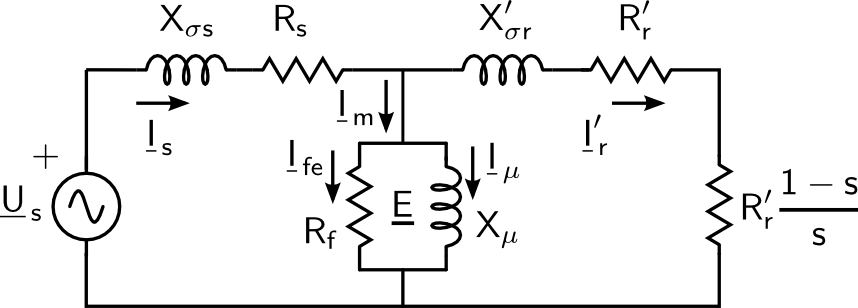
\includegraphics[scale=1.5]{png/mi_circ_math.png} 


    \subsection{Circuito equivalente (variables python)}


    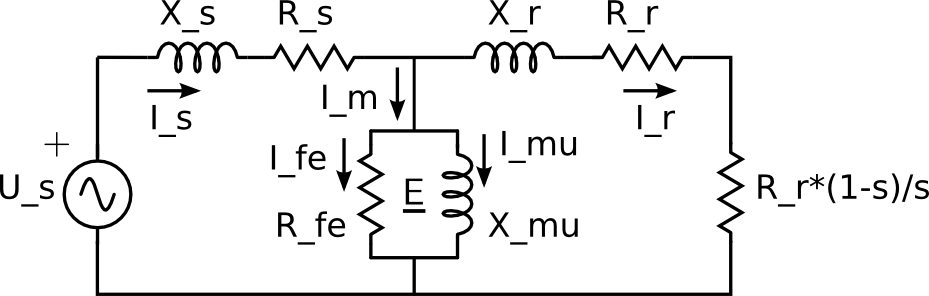
\includegraphics[scale=1.5]{png/mi_circ_py.png} 


    

    \subsubsection{Deslizamiento porcentual}

    Con la frecuencia:

\[ \sf f = 50 \; H_z\]

Y los pares de polo se puede calcular la velocidad síncrona:

\[ \sf \Omega_1 = \frac{2 \pi f}{N_{pp}} [=] \frac{r}{s}\]

La velocidad de giro del eje se puede obtener a partir de la velocidad
dada en revoluciones por minuto:

\[ \sf \Omega =  \frac{n \cdot 2 \pi}{60} [=] \frac{r}{s} \]

Deslizamiento:

\[ \sf s = \frac{\Omega_1 - \Omega}{\Omega_1}\]

Deslizamiento porcentual:

\[ \sf s_{\%} = s \cdot 100\]

    \begin{Verbatim}[commandchars=\\\{\}]
{\color{incolor}In [{\color{incolor}12}]:} \PY{k+kn}{import} \PY{n+nn}{numpy} \PY{k+kn}{as} \PY{n+nn}{np}
         \PY{n}{N\PYZus{}pp} \PY{o}{=} \PY{l+m+mi}{2}
         \PY{n}{f} \PY{o}{=} \PY{l+m+mf}{50.0}
         \PY{n}{n} \PY{o}{=} \PY{l+m+mf}{1470.0}
         
         \PY{n}{Omega\PYZus{}1} \PY{o}{=} \PY{l+m+mf}{2.0}\PY{o}{*}\PY{n}{np}\PY{o}{.}\PY{n}{pi}\PY{o}{*}\PY{l+m+mf}{50.0}\PY{o}{/}\PY{n}{N\PYZus{}pp}
         \PY{n}{Omega} \PY{o}{=} \PY{l+m+mf}{2.0}\PY{o}{*}\PY{n}{np}\PY{o}{.}\PY{n}{pi}\PY{o}{*}\PY{n}{n}\PY{o}{/}\PY{l+m+mf}{60.0}
         \PY{n}{s} \PY{o}{=} \PY{p}{(}\PY{n}{Omega\PYZus{}1} \PY{o}{\PYZhy{}} \PY{n}{Omega}\PY{p}{)}\PY{o}{/}\PY{p}{(}\PY{n}{Omega\PYZus{}1}\PY{p}{)}
         \PY{n}{s\PYZus{}porcentual} \PY{o}{=} \PY{n}{s}\PY{o}{*}\PY{l+m+mf}{100.0}
\end{Verbatim}

    \begin{Verbatim}[commandchars=\\\{\}]
{\color{incolor}In [{\color{incolor}13}]:} \PY{k}{print}\PY{p}{(}\PY{l+s}{\PYZsq{}}\PY{l+s}{Deslizamiento porcentual: \PYZob{}:2.2f\PYZcb{} }\PY{l+s}{\PYZpc{}}\PY{l+s}{\PYZsq{}}\PY{o}{.}\PY{n}{format}\PY{p}{(}\PY{n}{s\PYZus{}porcentual}\PY{p}{)}\PY{p}{)}
\end{Verbatim}

    \begin{Verbatim}[commandchars=\\\{\}]
Deslizamiento porcentual: 2.00 \%
    \end{Verbatim}

    \subsubsection{Par útil a 1470 rpm}

    Con los parametros y el deslizamiento calculado se obtienen las
impedancias del estator y el rotor:

\[ \sf \underline Z_s = R_s + j X_s \]

\[ \sf \underline Z_r = \frac{R_r}{s}  + jX_r\]

    La impedancia equivalente de la rama de magnetización:

\[ \sf  \underline Z_m = \frac{R_f \cdot jX_\mu}{R_f + jX_\mu} \]

Con la impedancia rotorica y la de la rama de magnetización se puede
obtener una impedancia equivalente magnetización-rotor:

\[ \sf  \underline Z_{mr} = \frac{\underline Z_m  \underline Z_r}{ \underline Z_m +  \underline Z_r}\]

La impedancia equivalente de todo el circuito se obtiene sumando la
impedancia estatorica y la impedancia equivalente rotor-estator:

\[ \sf  \underline Z_{eq} = \underline Z_s +  \underline Z_{mr} \]

    \begin{Verbatim}[commandchars=\\\{\}]
{\color{incolor}In [{\color{incolor}14}]:} \PY{n}{R\PYZus{}s}\PY{p}{,} \PY{n}{X\PYZus{}s} \PY{o}{=} \PY{l+m+mf}{0.17}\PY{p}{,} \PY{l+m+mf}{0.35}   \PY{c}{\PYZsh{} Ω }
         \PY{n}{R\PYZus{}f}\PY{p}{,} \PY{n}{X\PYZus{}mu} \PY{o}{=} \PY{l+m+mf}{347.0}\PY{p}{,} \PY{l+m+mf}{17.3} \PY{c}{\PYZsh{} Ω}
         \PY{n}{R\PYZus{}r}\PY{p}{,} \PY{n}{X\PYZus{}r} \PY{o}{=} \PY{l+m+mf}{0.12}\PY{p}{,} \PY{l+m+mf}{1.06}   \PY{c}{\PYZsh{} Ω    }
         
         \PY{n}{Z\PYZus{}s} \PY{o}{=} \PY{n}{R\PYZus{}s} \PY{o}{+} \PY{l+m+mi}{1j}\PY{o}{*}\PY{n}{X\PYZus{}s}
         \PY{n}{Z\PYZus{}m} \PY{o}{=} \PY{p}{(}\PY{n}{R\PYZus{}f} \PY{o}{*} \PY{l+m+mi}{1j}\PY{o}{*}\PY{n}{X\PYZus{}mu}\PY{p}{)} \PY{o}{/} \PY{p}{(}\PY{n}{R\PYZus{}f} \PY{o}{+} \PY{l+m+mi}{1j}\PY{o}{*}\PY{n}{X\PYZus{}mu}\PY{p}{)}
         \PY{n}{Z\PYZus{}r} \PY{o}{=} \PY{n}{R\PYZus{}r}\PY{o}{/}\PY{n}{s} \PY{o}{+} \PY{l+m+mi}{1j}\PY{o}{*}\PY{n}{X\PYZus{}r}
         
         \PY{n}{Z\PYZus{}mr} \PY{o}{=} \PY{n}{Z\PYZus{}m}\PY{o}{*}\PY{n}{Z\PYZus{}r}\PY{o}{/}\PY{p}{(}\PY{n}{Z\PYZus{}m} \PY{o}{+} \PY{n}{Z\PYZus{}r}\PY{p}{)}
         \PY{n}{Z\PYZus{}eq} \PY{o}{=} \PY{n}{Z\PYZus{}s} \PY{o}{+} \PY{n}{Z\PYZus{}mr}
\end{Verbatim}

    \[ \sf  \underline U_s =\frac{400}{\sqrt 3} \angle{ 0^\circ}  V\]

\[ \sf  \underline I_s = \frac{ \underline U_s}{ \underline Z_{eq}}\]

    \subsubsection{Corriente estatorica a 1470 rpm}

    \begin{Verbatim}[commandchars=\\\{\}]
{\color{incolor}In [{\color{incolor}15}]:} \PY{n}{U\PYZus{}s} \PY{o}{=} \PY{l+m+mf}{400.0}\PY{o}{/}\PY{n}{np}\PY{o}{.}\PY{n}{sqrt}\PY{p}{(}\PY{l+m+mf}{3.0}\PY{p}{)}
         \PY{n}{I\PYZus{}s} \PY{o}{=} \PY{n}{U\PYZus{}s}\PY{o}{/}\PY{n}{Z\PYZus{}eq}
\end{Verbatim}

    \begin{Verbatim}[commandchars=\\\{\}]
{\color{incolor}In [{\color{incolor}16}]:} \PY{k}{print}\PY{p}{(}\PY{l+s}{\PYZsq{}}\PY{l+s}{La corriente  = \PYZob{}:2.2f\PYZcb{} A}\PY{l+s}{\PYZsq{}}\PY{o}{.}\PY{n}{format}\PY{p}{(}\PY{n}{np}\PY{o}{.}\PY{n}{abs}\PY{p}{(}\PY{n}{I\PYZus{}s}\PY{p}{)}\PY{p}{)}\PY{p}{)}
\end{Verbatim}

    \begin{Verbatim}[commandchars=\\\{\}]
La corriente  = 40.51 A
    \end{Verbatim}

    \[ \sf  \underline E =  \underline U_s -  \underline Z_s  \underline I_s\]

\[ \sf  \underline I_r = \frac{ \underline E}{ \underline Z_r}\]

    \begin{Verbatim}[commandchars=\\\{\}]
{\color{incolor}In [{\color{incolor}17}]:} \PY{n}{E} \PY{o}{=} \PY{n}{U\PYZus{}s} \PY{o}{\PYZhy{}} \PY{n}{Z\PYZus{}s}\PY{o}{*}\PY{n}{I\PYZus{}s}
         \PY{n}{I\PYZus{}r} \PY{o}{=} \PY{n}{E}\PY{o}{/}\PY{n}{Z\PYZus{}r}
\end{Verbatim}

    \begin{Verbatim}[commandchars=\\\{\}]
{\color{incolor}In [{\color{incolor}18}]:} \PY{c}{\PYZsh{}\PYZsh{}\PYZsh{} Par útil a 1470 rpm }
\end{Verbatim}

    \[ \sf P_{mi} = 3 R_r  \frac{\left( 1-s \right)}  {s} \vert  \underline I_r\vert ^2\]
\[ \sf P_u = P_{mi} \]

\[ \sf T_u = \frac{P_u}{\Omega}\]

    \begin{Verbatim}[commandchars=\\\{\}]
{\color{incolor}In [{\color{incolor}19}]:} \PY{n}{P\PYZus{}mi} \PY{o}{=} \PY{l+m+mf}{3.0}\PY{o}{*}\PY{n}{R\PYZus{}r}\PY{o}{*}\PY{p}{(}\PY{l+m+mf}{1.0}\PY{o}{\PYZhy{}}\PY{n}{s}\PY{p}{)}\PY{o}{/}\PY{n}{s}\PY{o}{*}\PY{p}{(}\PY{n}{np}\PY{o}{.}\PY{n}{abs}\PY{p}{(}\PY{n}{I\PYZus{}r}\PY{p}{)}\PY{o}{*}\PY{o}{*}\PY{l+m+mi}{2}\PY{p}{)}
         \PY{n}{P\PYZus{}u} \PY{o}{=} \PY{n}{P\PYZus{}mi} \PY{c}{\PYZsh{} en el caso en el que las pérdidas fueron incluidas en R\PYZus{}f}
         
         \PY{n}{T\PYZus{}u} \PY{o}{=} \PY{n}{P\PYZus{}u}\PY{o}{/}\PY{n}{Omega}
\end{Verbatim}

    \begin{Verbatim}[commandchars=\\\{\}]
{\color{incolor}In [{\color{incolor}20}]:} \PY{k}{print}\PY{p}{(}\PY{l+s}{\PYZsq{}}\PY{l+s}{El par T\PYZus{}u = \PYZob{}:2.2f\PYZcb{} N.m}\PY{l+s}{\PYZsq{}}\PY{o}{.}\PY{n}{format}\PY{p}{(}\PY{n}{T\PYZus{}u}\PY{p}{)}\PY{p}{)}
\end{Verbatim}

    \begin{Verbatim}[commandchars=\\\{\}]
El par T\_u = 146.78 N.m
    \end{Verbatim}

    \subsubsection{Corriente de arranque (s=1)}

    En el arranque el deslizamiento es:

\[ \sf s = 1\]

Con lo que se obtiene la siguiente impedancia rotórica:

\[ \sf \underline Z_r = R_r  + jX_r\]

La impedancia equivalente de la rama de magnetización:

\[ \sf  \underline Z_m = \frac{R_f \cdot jX_\mu}{R_f + jX_\mu} \]

Con la impedancia rotorica y la de la rama de magnetización se puede
obtener una impedancia equivalente magnetización-rotor:

\[ \sf  \underline Z_{mr} = \frac{\underline Z_m  \underline Z_r}{ \underline Z_m +  \underline Z_r}\]

La impedancia equivalente de todo el circuito se obtiene sumando la
impedancia estatorica y la impedancia equivalente rotor-estator:

\[ \sf  \underline Z_{eq} = \underline Z_s +  \underline Z_{mr} \]

    \begin{Verbatim}[commandchars=\\\{\}]
{\color{incolor}In [{\color{incolor}21}]:} \PY{n}{Z\PYZus{}s} \PY{o}{=} \PY{n}{R\PYZus{}s} \PY{o}{+} \PY{l+m+mi}{1j}\PY{o}{*}\PY{n}{X\PYZus{}s}
         \PY{n}{Z\PYZus{}m} \PY{o}{=} \PY{p}{(}\PY{n}{R\PYZus{}f} \PY{o}{*} \PY{l+m+mi}{1j}\PY{o}{*}\PY{n}{X\PYZus{}mu}\PY{p}{)} \PY{o}{/} \PY{p}{(}\PY{n}{R\PYZus{}f} \PY{o}{+} \PY{l+m+mi}{1j}\PY{o}{*}\PY{n}{X\PYZus{}mu}\PY{p}{)}
         \PY{n}{Z\PYZus{}r} \PY{o}{=} \PY{n}{R\PYZus{}r} \PY{o}{+} \PY{l+m+mi}{1j}\PY{o}{*}\PY{n}{X\PYZus{}r}
         
         \PY{n}{Z\PYZus{}mr} \PY{o}{=} \PY{n}{Z\PYZus{}m}\PY{o}{*}\PY{n}{Z\PYZus{}r}\PY{o}{/}\PY{p}{(}\PY{n}{Z\PYZus{}m} \PY{o}{+} \PY{n}{Z\PYZus{}r}\PY{p}{)}
         \PY{n}{Z\PYZus{}eq} \PY{o}{=} \PY{n}{Z\PYZus{}s} \PY{o}{+} \PY{n}{Z\PYZus{}mr}
         
         \PY{n}{U\PYZus{}s} \PY{o}{=} \PY{l+m+mf}{400.0}\PY{o}{/}\PY{n}{np}\PY{o}{.}\PY{n}{sqrt}\PY{p}{(}\PY{l+m+mf}{3.0}\PY{p}{)}
         \PY{n}{I\PYZus{}s} \PY{o}{=} \PY{n}{U\PYZus{}s}\PY{o}{/}\PY{n}{Z\PYZus{}eq}
\end{Verbatim}

    \begin{Verbatim}[commandchars=\\\{\}]
{\color{incolor}In [{\color{incolor}22}]:} \PY{k}{print}\PY{p}{(}\PY{l+s}{\PYZsq{}}\PY{l+s}{La corriente en el arranque = \PYZob{}:2.2f\PYZcb{} A}\PY{l+s}{\PYZsq{}}\PY{o}{.}\PY{n}{format}\PY{p}{(}\PY{n}{np}\PY{o}{.}\PY{n}{abs}\PY{p}{(}\PY{n}{I\PYZus{}s}\PY{p}{)}\PY{p}{)}\PY{p}{)}
\end{Verbatim}

    \begin{Verbatim}[commandchars=\\\{\}]
La corriente en el arranque = 167.65 A
    \end{Verbatim}


    % Add a bibliography block to the postdoc
    
    
    
    \end{document}
